\documentclass[10pt,letterpaper]{article}
% Kamiak cluster architecture -- compile with ./compile.sh (runs make_figs.py first)

\usepackage[T1]{fontenc}
\usepackage{montserrat}          % headings only, via \display; must load before opensans
\usepackage[default,scale=0.95]{opensans}
\usepackage[scale=0.88]{sourcecodepro}
\renewcommand{\sfdefault}{opensans-TLF}\renewcommand{\familydefault}{\sfdefault}
\usepackage{float}
\makeatletter\def\bfseries@sf{b}\def\mdseries@sf{m}\makeatother % montserrat renames these; opensans uses b/m
\usepackage[margin=1.9cm,top=1.7cm,bottom=1.9cm]{geometry}
\usepackage{xcolor}
\usepackage{tikz}
\usetikzlibrary{arrows.meta,positioning,calc,patterns,decorations.pathreplacing,backgrounds}
\usepackage{pgfplots}
\pgfplotsset{compat=1.18}
\pgfkeys{/pgf/number format/.cd,assume math mode=true,1000 sep={,}} % numbers in the text font, not CM math
\usepgfplotslibrary{groupplots}
\usepackage{booktabs,tabularx,array}
\usepackage{microtype}
\usepackage{enumitem}
\usepackage{titlesec}
\usepackage{caption}
\usepackage{fancyhdr}
\usepackage[hidelinks]{hyperref}

% ---------------------------------------------------------------- WSU colours
\definecolor{crimson}{HTML}{981E32}       % WSU crimson
\definecolor{crimsondark}{HTML}{6B1523}
\definecolor{crimsontint}{HTML}{F3DFE3}
\definecolor{wsugray}{HTML}{5E6A71}       % WSU gray
\definecolor{graymid}{HTML}{9AA3A8}
\definecolor{graylight}{HTML}{CDD2D5}
\definecolor{graypale}{HTML}{EEF0F1}
\definecolor{ink}{HTML}{1F2427}
\color{ink}

\newcommand{\display}{\fontfamily{Montserrat-TLF}\selectfont}
\newcommand{\yours}{{\color{crimson}\textbullet}}

% ---------------------------------------------------------------- layout
\setlength{\parindent}{0pt}
\setlength{\parskip}{6pt}
\linespread{1.08}
\titleformat{\section}{\display\Large\bfseries\color{ink}}{\color{crimson}\thesection}{0.6em}{}
\titlespacing*{\section}{0pt}{16pt}{6pt}
\titleformat{\subsection}{\display\normalsize\bfseries\color{ink}}{}{0pt}{}
\titlespacing*{\subsection}{0pt}{10pt}{3pt}
\captionsetup{font={small,color=wsugray},labelfont={bf,color=ink},labelsep=period,justification=raggedright,singlelinecheck=false,skip=6pt}
\setlist{itemsep=3pt,topsep=3pt,leftmargin=1.3em}
\pagestyle{fancy}\fancyhf{}
\renewcommand{\headrulewidth}{0pt}
\fancyfoot[L]{\scriptsize\color{wsugray}Kamiak cluster architecture \textperiodcentered{} October 2026}
\fancyfoot[R]{\scriptsize\color{wsugray}\thepage}

% ---------------------------------------------------------------- TikZ styles
\tikzset{
  zone/.style={font=\ttfamily\scriptsize\bfseries,text=wsugray,inner sep=0pt},
  box/.style={draw=graylight,fill=white,line width=0.6pt,rounded corners=1.5pt},
  dashedbox/.style={dash pattern=on 3pt off 2pt,draw=graymid},
  title/.style={font=\sffamily\footnotesize\bfseries,text=ink,inner sep=1pt},
  sub/.style={font=\sffamily\scriptsize,text=wsugray,inner sep=1pt},
  group/.style={draw=graymid,line width=0.6pt,rounded corners=3pt},
  server/.style={draw=graymid,fill=graypale,line width=0.4pt},
  bay/.style={fill=graylight},
  ledc/.style={fill=crimson},
  plain/.style={draw=graymid,line width=0.8pt},
  ib/.style={draw=crimson,line width=1.6pt},
  net/.style={draw=wsugray,line width=1.2pt},
  ctl/.style={draw=ink,line width=0.7pt},
  jobstep/.style={circle,fill=ink,text=white,font=\ttfamily\scriptsize\bfseries,inner sep=0pt,minimum size=11pt},
  rack/.style={draw=graymid,line width=0.6pt},
  slab/.style={fill=graylight},
  slabbig/.style={fill=wsugray},
  slabgpu/.style={fill=crimson},
  stripyou/.style={fill=crimson},
  stripyoubig/.style={fill=crimsondark},
  stripother/.style={fill=graylight},
  bracket/.style={draw=graymid,line width=0.6pt},
  bracketc/.style={draw=crimson,line width=0.9pt},
  leader/.style={draw=graymid,line width=0.4pt},
  lane/.style={draw=graylight,line width=0.6pt,dash pattern=on 2pt off 2pt},
  msg/.style={draw=ink,line width=0.7pt,-{Stealth[length=5pt]}},
  ret/.style={draw=wsugray,line width=0.6pt,dash pattern=on 3pt off 2pt,-{Stealth[length=4pt]}},
  data/.style={draw=crimson,line width=1.2pt,-{Stealth[length=5pt]}},
  lbl/.style={font=\sffamily\scriptsize,text=ink,fill=white,inner sep=1.5pt},
}

% ---------------------------------------------------------------- pgfplots
\pgfplotsset{
  wsubar/.style={
    xbar, bar width=7.5pt, bar shift=0pt,
    axis line style={draw=none}, tick style={draw=none},
    xmajorgrids, grid style={draw=graypale,line width=0.6pt},
    xmin=0, enlarge y limits=0.09,
    yticklabel style={font=\sffamily\scriptsize,text=ink},
    xticklabel style={font=\sffamily\scriptsize,text=wsugray},
    title style={font=\display\footnotesize\bfseries,text=ink,anchor=south west,at={(0,1.0)},xshift=-2pt},
    nodes near coords, nodes near coords align={horizontal},
    every node near coord/.style={font=\sffamily\scriptsize,text=ink,xshift=1pt},
    scaled x ticks=false,
    xticklabel={\pgfmathprintnumber[1000 sep={,}]{\tick}},
  },
}

\begin{document}

% ================================================================ title block
\begin{tikzpicture}[remember picture,overlay]
  \fill[crimson] (current page.north west) rectangle ([yshift=-0.55cm]current page.north east);
\end{tikzpicture}
\vspace*{2pt}
{\ttfamily\footnotesize\color{wsugray}WSU \textperiodcentered{} CENTER FOR INSTITUTIONAL RESEARCH COMPUTING \textperiodcentered{} KAMIAK}\par\vspace{4pt}
{\display\fontsize{30}{32}\selectfont\bfseries Kamiak Cluster Architecture\par}
\vspace{6pt}
{\large\color{wsugray}How the machines behind \texttt{ssh kamiak} fit together, and what that means for your jobs\par}
\vspace{14pt}

% key numbers
\newcommand{\stat}[2]{\begin{minipage}[t]{0.19\textwidth}{\display\fontsize{20}{22}\selectfont\bfseries\color{crimson}#1}\\[1pt]{\scriptsize\color{wsugray}#2}\end{minipage}}
\noindent\stat{146}{compute nodes}\hfill\stat{7,136}{CPU cores}\hfill\stat{20}{GPUs on 6 nodes}\hfill\stat{1\,PB}{all-flash WekaIO storage}\hfill\stat{100\,Gb/s}{InfiniBand HDR100}
\vspace{6pt}
{\color{graylight}\rule{\textwidth}{0.6pt}}

\section{The whole system}

Kamiak is a \emph{condominium} cluster. Faculty investors and colleges buy compute nodes; WSU provides the head nodes, the network, the storage and the staff. Every machine plugs into one InfiniBand fabric, so a file written anywhere appears everywhere, and a job can spread across nodes. Figure~\ref{fig:system} shows each of the 146 compute nodes as one slab, grouped by the partition that owns it.

\begin{figure}[H]
\centering
\input{figs/system.tex}
\caption{Kamiak's hardware and the path of one job (\textbf{1}--\textbf{5}, detailed in Figure~\ref{fig:job}). Racks are grouped by partition, not by physical position. The number of Weka storage servers is illustrative; CIRC does not publish it.}
\label{fig:system}
\end{figure}

\section{Compute nodes}

The nodes span ten years of Intel Xeon generations. Most \emph{nodes} are old, but most \emph{cores} are new: the 50 Sapphire Rapids and Granite Rapids nodes, the generations \texttt{popov} is built from, hold 57\% of the cluster's cores.

\begin{figure}[H]
\centering
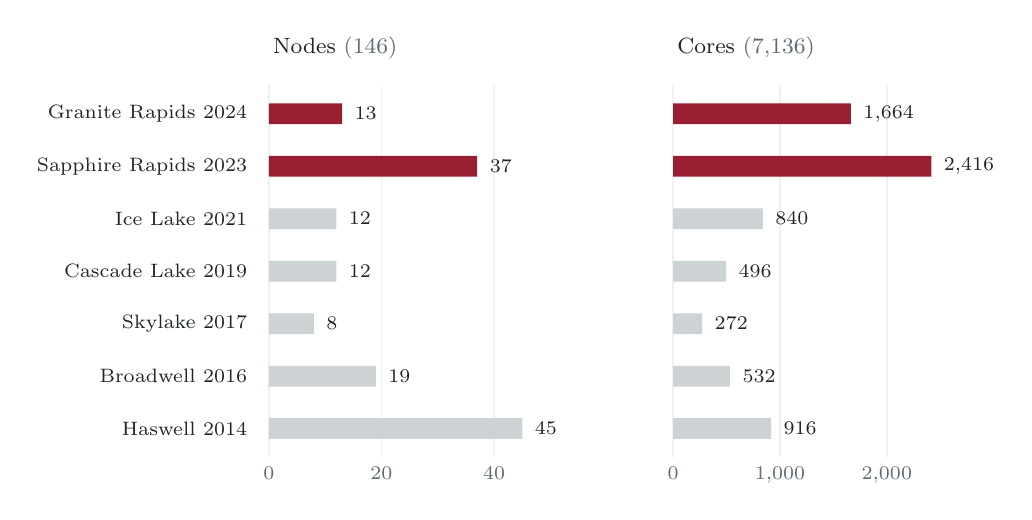
\begin{tikzpicture}
\begin{groupplot}[group style={group size=2 by 1, horizontal sep=1.2cm, yticklabels at=edge left},
  wsubar, width=0.455\textwidth, height=6.3cm,
  symbolic y coords={has,bro,sky,cas,ice,spr,gnr}, ytick={has,bro,sky,cas,ice,spr,gnr},
  yticklabels={Haswell 2014,Broadwell 2016,Skylake 2017,Cascade Lake 2019,Ice Lake 2021,Sapphire Rapids 2023,Granite Rapids 2024}]
\nextgroupplot[title={Nodes \textcolor{wsugray}{\mdseries (146)}}, xmax=55]
  \addplot[fill=graylight,draw=none] coordinates {(45,has) (19,bro) (8,sky) (12,cas) (12,ice)};
  \addplot[fill=crimson,draw=none] coordinates {(37,spr) (13,gnr)};
\nextgroupplot[title={Cores \textcolor{wsugray}{\mdseries (7,136)}}, xmax=2900]
  \addplot[fill=graylight,draw=none] coordinates {(916,has) (532,bro) (272,sky) (496,cas) (840,ice)};
  \addplot[fill=crimson,draw=none] coordinates {(2416,spr) (1664,gnr)};
\end{groupplot}
\end{tikzpicture}
\caption{Kamiak by CPU generation (year of the Xeon generation's launch). Crimson marks the two newest generations: 34\% of nodes, 57\% of cores. Haswell is the reverse: 31\% of nodes, 13\% of cores. Source: hpc.wsu.edu partition list.}
\label{fig:gen}
\end{figure}

\begin{minipage}[t]{0.47\textwidth}
\subsection{Inside \texttt{popov}}
\small
\begin{tabularx}{\linewidth}{@{}l r r X@{}}
\toprule
\textbf{Nodes} & \textbf{Cores} & \textbf{RAM*} & \textbf{CPU}\\
\midrule
\texttt{cn154--168} (15) & 64 & 100\,GB & Sapphire Rapids\\
\texttt{cn177--182} (6) & 128 & 151\,GB & Granite Rapids\\
\bottomrule
\end{tabularx}\par\vspace{3pt}
{\scriptsize\color{wsugray}*Memory Slurm lets a job request, from \texttt{sinfo}, June 2026. A 64-core, $\le$100\,GB request can start on all 21 nodes; a 128-core request only on 6.}
\end{minipage}\hfill
\begin{minipage}[t]{0.47\textwidth}
\subsection{GPUs}
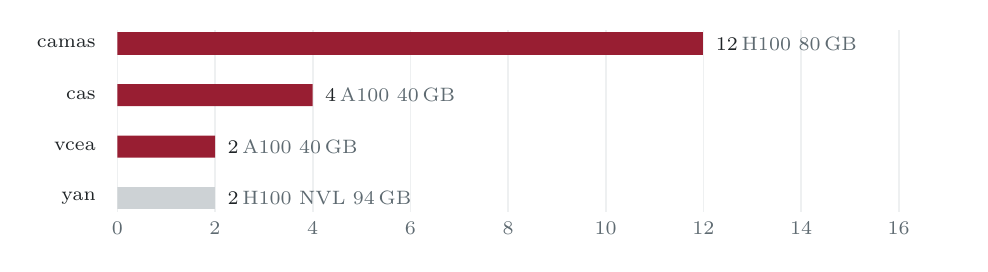
\begin{tikzpicture}
\begin{axis}[wsubar, width=\linewidth, height=3.9cm, xmax=17, bar width=8pt,
  symbolic y coords={yan,vcea,cas,camas}, ytick={yan,vcea,cas,camas}]
  \addplot[fill=crimson,draw=none,nodes near coords={12\,\textcolor{wsugray}{H100 80\,GB}}] coordinates {(12,camas)};
  \addplot[fill=crimson,draw=none,nodes near coords={\pgfmathprintnumber{\pgfplotspointmeta}\,\textcolor{wsugray}{A100 40\,GB}}] coordinates {(4,cas) (2,vcea)};
  \addplot[fill=graylight,draw=none,nodes near coords={2\,\textcolor{wsugray}{H100 NVL 94\,GB}}] coordinates {(2,yan)};
\end{axis}
\end{tikzpicture}\par
{\scriptsize\color{wsugray}GPUs per partition. Crimson: partitions in your banner. Only \texttt{camas} is open to everyone, and GPU jobs there are never preempted.}
\end{minipage}

\section{Partitions are labels on nodes}

A partition is not a separate machine; it is a list of nodes. The same \texttt{popov} node is also a \texttt{kamiak} node, because the backfill partition covers every node on the cluster (Figure~\ref{fig:strip}). That overlap is what makes \texttt{kamiak} free to use, and it is also why jobs there can be killed.

\begin{figure}[H]
\centering
\input{figs/strip.tex}
\caption{All 146 compute nodes in a row. Crimson: partitions in your banner (darker: \texttt{popov}'s 128-core nodes). Dots: GPU nodes. Every node sits in its owner's partition \emph{and} in \texttt{kamiak}. \texttt{dtn} (data transfer) is not drawn; its nodes are not published.}
\label{fig:strip}
\end{figure}

\subsection{What preemption does to one node}

When an owner needs cores that a backfill job holds, Slurm cancels the backfill job and puts it back in the \texttt{kamiak} queue. The work done since the last restart file is lost.

\begin{figure}[H]
\centering
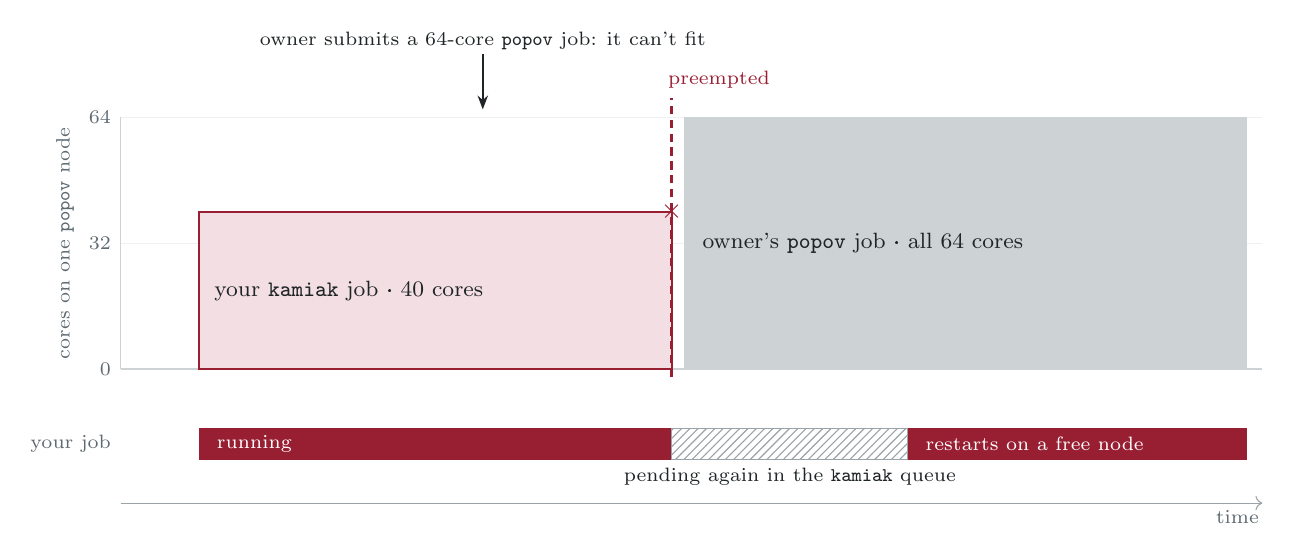
\begin{tikzpicture}[x=1cm,y=1cm,font=\sffamily\scriptsize]
  % axes
  \draw[graylight,line width=0.6pt] (0,0) -- (14.5,0);
  \draw[graylight,line width=0.6pt] (0,0) -- (0,3.2);
  \foreach \c/\y in {0/0,32/1.6,64/3.2} {\node[sub,anchor=east] at (-0.08,\y) {\c};}
  \draw[graypale,line width=0.5pt] (0,1.6) -- (14.5,1.6) (0,3.2) -- (14.5,3.2);
  \node[sub,rotate=90,anchor=south] at (-0.55,1.6) {cores on one \texttt{popov} node};
  % your job
  \fill[crimsontint] (1,0) rectangle (7,2.0);
  \draw[crimson,line width=0.8pt] (1,0) rectangle (7,2.0);
  \node[title,anchor=west] at (1.15,1.0) {your \texttt{kamiak} job \textperiodcentered{} 40 cores};
  % owner submits
  \draw[msg] (4.6,4.0) -- (4.6,3.3);
  \node[lbl,anchor=south] at (4.6,4.0) {owner submits a 64-core \texttt{popov} job: it can't fit};
  % preemption
  \draw[crimson,line width=1pt,dash pattern=on 3pt off 2pt] (7,-0.1) -- (7,3.45);
  \node[font=\sffamily\scriptsize\bfseries,text=crimson,anchor=south] at (7.6,3.45) {preempted};
  \node[text=crimson,font=\bfseries] at (7,2.0) {$\times$};
  % owner job
  \fill[graylight] (7.15,0) rectangle (14.3,3.2);
  \node[title,anchor=west] at (7.35,1.6) {owner's \texttt{popov} job \textperiodcentered{} all 64 cores};
  % your job's own lane
  \node[sub,anchor=east] at (-0.08,-0.95) {your job};
  \fill[crimson] (1,-1.15) rectangle (7,-0.75);
  \node[font=\sffamily\scriptsize,text=white,anchor=west] at (1.1,-0.95) {running};
  \fill[pattern=north east lines,pattern color=graymid] (7,-1.15) rectangle (10,-0.75);
  \draw[graymid,line width=0.5pt] (7,-1.15) rectangle (10,-0.75);
  \node[lbl,anchor=north] at (8.5,-1.2) {pending again in the \texttt{kamiak} queue};
  \fill[crimson] (10,-1.15) rectangle (14.3,-0.75);
  \node[font=\sffamily\scriptsize,text=white,anchor=west] at (10.1,-0.95) {restarts on a free node};
  \draw[->,graymid] (0,-1.7) -- (14.5,-1.7) node[sub,anchor=north east] at (14.5,-1.75) {time};
\end{tikzpicture}
\caption{Preemption on one 64-core \texttt{popov} node. The node does not change; only who holds its cores. A job that writes restart files resumes where it left off; one that doesn't starts over.}
\label{fig:preempt}
\end{figure}

\section{Storage: one filesystem, many servers}

\texttt{/home}, \texttt{/data/lab} and \texttt{/scratch} are not on the login nodes or the compute nodes. They live on WekaFS, a parallel filesystem: each file is cut into chunks spread across many flash servers, with extra protection chunks so a failed drive or server loses nothing. Every node mounts it over InfiniBand, so it behaves like one local disk that every node shares.

\begin{figure}[H]
\centering
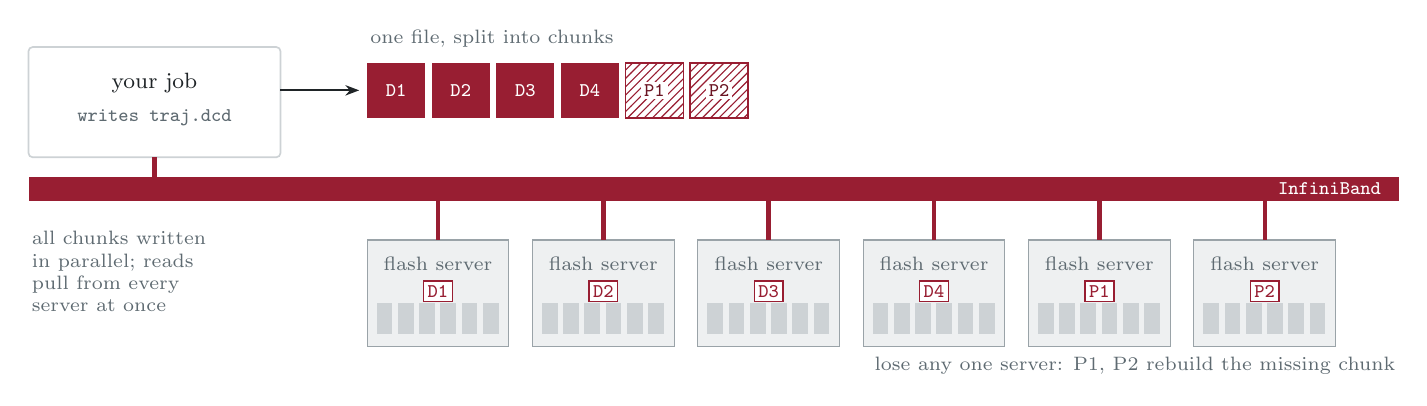
\begin{tikzpicture}[x=1cm,y=1cm,font=\sffamily\scriptsize]
  % job
  \node[box,minimum width=3.2cm,minimum height=1.4cm] (job) at (1.6,2.2) {};
  \node[title] at (1.6,2.45) {your job};
  \node[sub] at (1.6,2.0) {\ttfamily writes traj.dcd};
  % file split into chunks
  \node[sub,anchor=south west] at (4.3,2.85) {one file, split into chunks};
  \foreach \i in {0,...,3} {
    \fill[crimson] (4.3+\i*0.82,2.0) rectangle (5.04+\i*0.82,2.7);
    \pgfmathtruncatemacro{\n}{\i+1}
    \node[font=\ttfamily\scriptsize\bfseries,text=white] at (4.67+\i*0.82,2.35) {D\n};
  }
  \foreach \i in {0,1} {
    \fill[pattern=north east lines,pattern color=crimson] (7.58+\i*0.82,2.0) rectangle (8.32+\i*0.82,2.7);
    \draw[crimson,line width=0.6pt] (7.58+\i*0.82,2.0) rectangle (8.32+\i*0.82,2.7);
    \pgfmathtruncatemacro{\n}{\i+1}
    \node[font=\ttfamily\scriptsize\bfseries,text=crimsondark,fill=white,inner sep=1pt] at (7.95+\i*0.82,2.35) {P\n};
  }
  \draw[msg] (3.2,2.35) -- (4.2,2.35);
  % fabric
  \fill[crimson] (0,0.95) rectangle (17.4,1.25);
  \node[font=\ttfamily\scriptsize\bfseries,text=white,anchor=east] at (17.3,1.1) {InfiniBand};
  % servers
  \foreach \i/\c in {0/D1,1/D2,2/D3,3/D4,4/P1,5/P2} {
    \pgfmathsetmacro{\x}{4.3+\i*2.1}
    \draw[server] (\x,-0.9) rectangle (\x+1.8,0.45);
    \foreach \j in {0,...,5} {\fill[bay] (\x+0.12+\j*0.27,-0.75) rectangle (\x+0.32+\j*0.27,-0.35);}
    \node[sub] at (\x+0.9,0.15) {flash server};
    \node[font=\ttfamily\scriptsize\bfseries,text=crimson] at (\x+0.9,-0.6) {};
    \draw[ib] (\x+0.9,0.45) -- (\x+0.9,0.95);
    \node[font=\ttfamily\scriptsize\bfseries,fill=white,text=crimson,inner sep=1.5pt,draw=crimson,line width=0.5pt] at (\x+0.9,-0.2) {\c};
  }
  \draw[ib] (1.6,1.5) -- (1.6,1.25);
  \node[sub,anchor=north west,align=left] at (0,0.6) {all chunks written\\in parallel; reads\\pull from every\\server at once};
  \node[sub,anchor=north east,align=right] at (17.4,-1.0) {lose any one server: P1, P2 rebuild the missing chunk};
\end{tikzpicture}
\caption{How WekaFS stores one file (illustrative: Kamiak's chunk and server counts are not published). Large reads and writes use every server at once; millions of tiny files are slower, because each one costs a metadata lookup.}
\label{fig:weka}
\end{figure}

\begin{table}[H]
\small
\begin{tabularx}{\textwidth}{@{}l l X l@{}}
\toprule
\textbf{Path} & \textbf{Size} & \textbf{Kept} & \textbf{On compute nodes}\\
\midrule
\texttt{/home} & 100\,GB per user & daily snapshots, kept 3 days & yes\\
\texttt{/data/lab} & 500\,GB per PI, more for rent & daily snapshots, kept 3 days & yes\\
\texttt{/scratch} & 10\,TB per user & workspaces deleted after 2 weeks (\texttt{mkworkspace}) & yes\\
\texttt{/archive} & rented & cold data & \textcolor{crimson}{\textbf{no}}: login and \texttt{dtn} only\\
\bottomrule
\end{tabularx}
\caption{Storage tiers. All share the same flash and the same speed; they differ in size and lifetime. Nothing is backed up off the cluster.}
\end{table}

\section{One job, start to finish}

\begin{figure}[H]
\centering
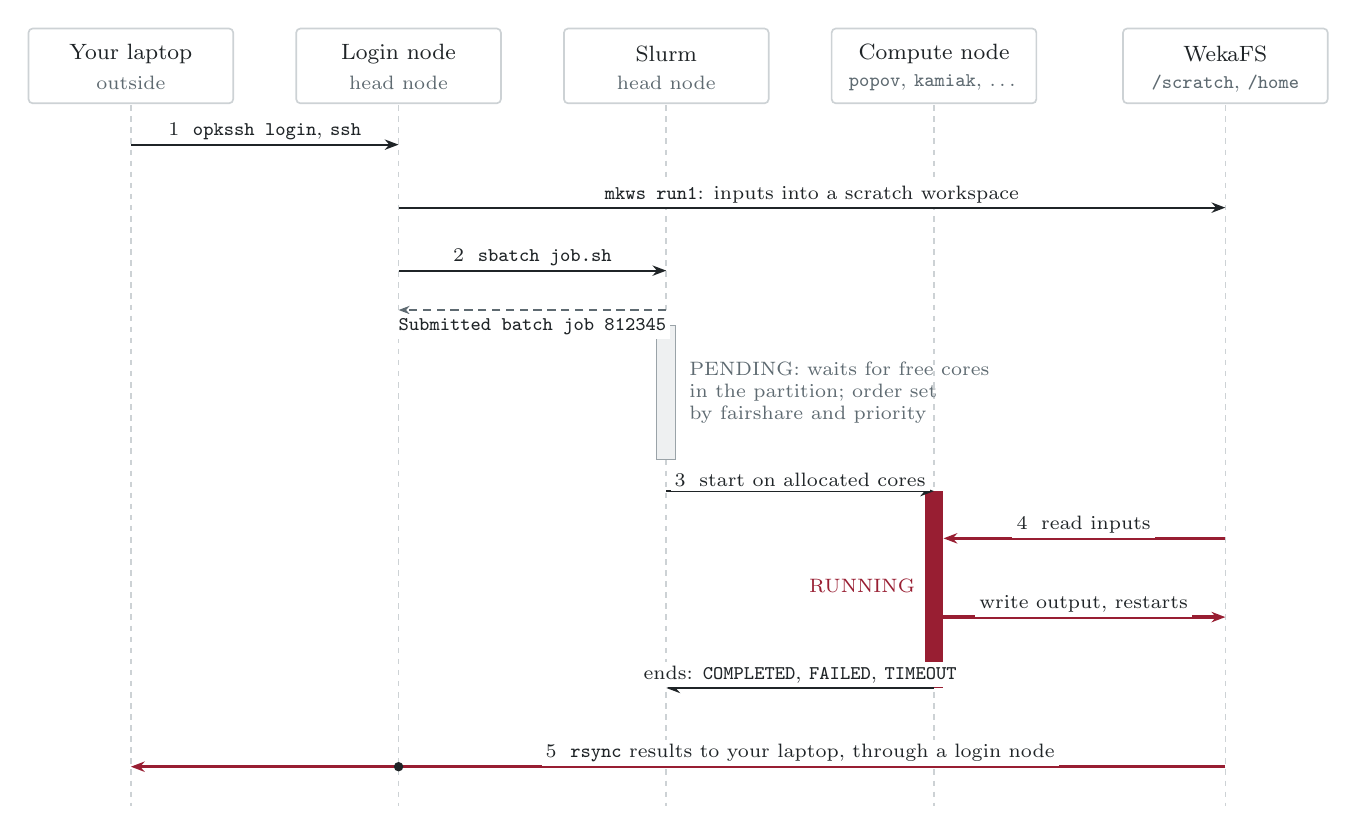
\begin{tikzpicture}[x=1cm,y=1cm,font=\sffamily\scriptsize]
  \foreach \x/\n/\s in {1.3/Your laptop/outside, 4.7/Login node/head node, 8.1/Slurm/head node, 11.5/Compute node/{\texttt{popov}, \texttt{kamiak}, \dots}, 15.2/WekaFS/{\texttt{/scratch}, \texttt{/home}}} {
    \node[box,minimum width=2.6cm,minimum height=0.95cm] at (\x,0) {};
    \node[title] at (\x,0.15) {\n};
    \node[sub] at (\x,-0.22) {\s};
    \draw[lane] (\x,-0.5) -- (\x,-9.4);
  }
  % activations
  \fill[graypale] (7.98,-3.3) rectangle (8.22,-5.0); \draw[graymid,line width=0.4pt] (7.98,-3.3) rectangle (8.22,-5.0);
  \fill[crimson] (11.38,-5.4) rectangle (11.62,-7.9);
  % messages
  \draw[msg] (1.3,-1.0) -- (4.7,-1.0);   \node[lbl,anchor=south] at (3.0,-1.0) {\textbf{1}\; \texttt{opkssh login}, \texttt{ssh}};
  \draw[msg] (4.7,-1.8) -- (15.2,-1.8);  \node[lbl,anchor=south] at (9.95,-1.8) {\texttt{mkws run1}: inputs into a scratch workspace};
  \draw[msg] (4.7,-2.6) -- (8.1,-2.6);   \node[lbl,anchor=south] at (6.4,-2.6) {\textbf{2}\; \texttt{sbatch job.sh}};
  \draw[ret] (8.1,-3.1) -- (4.7,-3.1);   \node[lbl,anchor=north] at (6.4,-3.15) {\texttt{Submitted batch job 812345}};
  \node[sub,anchor=west,align=left] at (8.35,-4.15) {\textbf{PENDING}: waits for free cores\\in the partition; order set\\by fairshare and priority};
  \draw[msg] (8.1,-5.4) -- (11.5,-5.4);  \node[lbl,anchor=south] at (9.8,-5.4) {\textbf{3}\; start on allocated cores};
  \node[sub,anchor=east,align=right,text=crimson] at (11.3,-6.6) {\textbf{RUNNING}};
  \draw[data] (15.2,-6.0) -- (11.62,-6.0); \node[lbl,anchor=south] at (13.4,-6.0) {\textbf{4}\; read inputs};
  \draw[data] (11.62,-7.0) -- (15.2,-7.0); \node[lbl,anchor=south] at (13.4,-7.0) {write output, restarts};
  \draw[msg] (11.5,-7.9) -- (8.1,-7.9);  \node[lbl,anchor=south] at (9.8,-7.9) {ends: \texttt{COMPLETED}, \texttt{FAILED}, \texttt{TIMEOUT}};
  \draw[data] (15.2,-8.9) -- (1.3,-8.9); \fill[ink] (4.7,-8.9) circle (0.06);
  \node[lbl,anchor=south] at (9.8,-8.9) {\textbf{5}\; \texttt{rsync} results to your laptop, through a login node};
\end{tikzpicture}
\caption{A batch job over time, top to bottom. Crimson arrows carry your data; black arrows are commands and scheduler events. Steps \textbf{1}--\textbf{5} match Figure~\ref{fig:system}.}
\label{fig:job}
\end{figure}

\section{Your partitions}

\begin{table}[H]
\small
\begin{tabularx}{\textwidth}{@{}l l l l X@{}}
\toprule
\textbf{Partition} & \textbf{Kind} & \textbf{Nodes} & \textbf{Preempted?} & \textbf{Notes}\\
\midrule
\texttt{kamiak} & backfill, open to all & 146 & \textcolor{crimson}{\textbf{yes}} & every node; use for short or checkpointed runs\\
\texttt{popov} & investor & 21 & no & no \texttt{-{}-exclusive}; ask for cores and \texttt{-{}-mem} instead\\
\texttt{camas} & NSF GPU, open to all & 3 (12 H100) & no, for GPU jobs & non-GPU jobs are moved to \texttt{kamiak}; cite NSF award CNS-2216108\\
\texttt{cas} & college & 13 (4 A100) & no & College of Arts and Sciences\\
\texttt{vcea} & college & 4 (2 A100) & no & Voiland College of Engineering and Architecture\\
\texttt{beckman} & investor & not published & no & size not published; \texttt{scontrol show partition} lists it\\
\texttt{dtn} & data transfer & not published & & large copies, and the only compute access to \texttt{/archive}\\
\bottomrule
\end{tabularx}
\caption{The partitions in your login banner. You can list several in one job, e.g.\ \texttt{\#SBATCH -p popov,kamiak}; Slurm starts it on whichever frees up first.}
\end{table}

\section{What this means for your research}

\begin{itemize}
\item \textbf{Run long jobs where they can't be killed.} Multi-day CP2K AIMD and umbrella-sampling windows belong on \texttt{popov}, not \texttt{kamiak}. Anything on \texttt{kamiak} should write restart files often (Figure~\ref{fig:preempt}).
\item \textbf{Size jobs to the hardware.} 64 cores and $\le$100\,GB fits all 21 \texttt{popov} nodes and starts soonest. For 64--100 atom cells, one node is the sweet spot; spreading across nodes adds InfiniBand traffic that rarely pays at that size.
\item \textbf{Use arrays for many similar runs.} Dozens of PMF windows or LAMMPS replicas go in one job array, as the login banner asks.
\item \textbf{Train ML potentials on \texttt{camas}.} Twelve H100s, open to all and not preempted for GPU jobs. Acknowledge NSF CNS-2216108 in papers that use them.
\item \textbf{Download before you submit.} Compute nodes have no internet: fetch pseudopotentials, basis sets, model weights and packages on a login node first.
\item \textbf{Keep files big and few.} WekaFS streams large trajectories fast; millions of small files are slow. Tar outputs, and keep conda environments out of \texttt{/scratch}.
\item \textbf{Move results out of \texttt{/scratch} within two weeks}, to \texttt{/data/lab}, and keep a copy off the cluster.
\item \textbf{Methods sections.} Report the CPU generation (Sapphire or Granite Rapids for \texttt{popov}), the HDR100 interconnect, and the CIRC acknowledgement: \emph{``This research used resources of the Center for Institutional Research Computing at Washington State University.''}
\end{itemize}

\vfill
{\color{graylight}\rule{\textwidth}{0.6pt}}\par
{\scriptsize\color{wsugray}
\textbf{Sources} (read 12 October 2026): hpc.wsu.edu pages \emph{Cluster Resources} (node, core, GPU, head-node, network and storage figures), \emph{Storage}, \emph{File Transfers}, \emph{Quick Start Guide}, \emph{Camas GPU Cluster} and \emph{Acceptable Use Policy}; \texttt{sinfo -p popov -N -l} (June 2026). Not published, and therefore not drawn: the management Ethernet network, the InfiniBand switch layout, physical rack positions, Weka server count, and node counts for investor partitions other than \texttt{popov}. Colours: WSU crimson \#981E32 and gray \#5E6A71.\par}

\end{document}
